\section{Förderband}
\label{sec:Foerderband}
    Die Ansteuerung des Motors, der das Förderband antreibt erfolgt mittels PWM. Auf diese 
    weise lässt sich die Drehzahl und somit die Nachführgeschwindigkeit einstellen. Das 
    Band muss nur ein eine Richtung angetrieben werden, wodurch die Ansteuerung einfacher 
    realisiert werden kann. Das Schema ist in Abbildung \ref{abb:SchemaAnsteuerung} 
    ersichtlich. Im wesentlichen besteht diese Ansteuerung aus einem Vortreiber und eines 
    Schalters. Der Treiber dient dazu, den Schalter möglichst schnell und effizient zu 
    öffnen und zu schliessen. Auf diese Weise reduziert man die Schaltverluste. 
    \begin{figure}[h!]
    	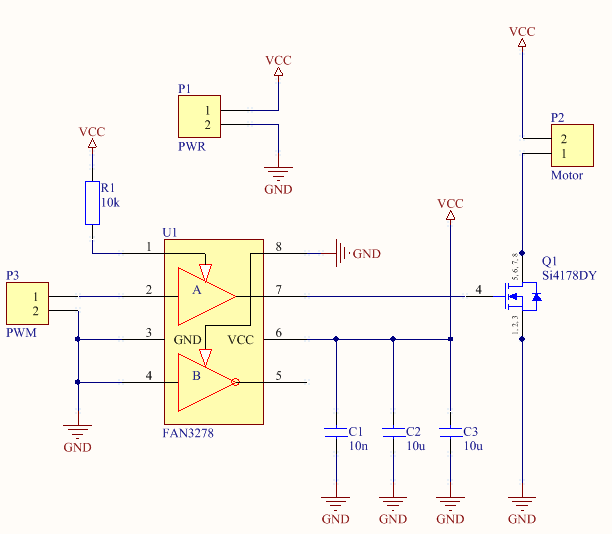
\includegraphics[width=0.4\textwidth,clip,trim=0mm 0mm 0mm 0mm]
    	{Enddokumentation/Bilder/Schema_DC-Ansteuerung.png}
    	\centering
    	\caption{Schema des Förderbandantriebes}
    	\label{abb:SchemaAnsteuerung}
    \end{figure}